%%%%%%%%%%%%%%%%%%%%%%%%%%%%%%%%%%%%%%%%%
% Dreuw & Deselaer's Poster
% LaTeX Template
% Version 1.0 (11/04/13)
%
% Created by:
% Philippe Dreuw and Thomas Deselaers
% http://www-i6.informatik.rwth-aachen.de/~dreuw/latexbeamerposter.php
% 
% This template has been downloaded from:
% http://www.LaTeXTemplates.com
%
% License:
% CC BY-NC-SA 3.0 (http://creativecommons.org/licenses/by-nc-sa/3.0/)
%
%%%%%%%%%%%%%%%%%%%%%%%%%%%%%%%%%%%%%%%%%

%----------------------------------------------------------------------------------------
%	PACKAGES AND OTHER DOCUMENT CONFIGURATIONS
%----------------------------------------------------------------------------------------

\documentclass[final,hyperref={pdfpagelabels=false}]{beamer}

%\setbeamercolor{block title}{fg=black,bg=orange!70} % Change the block title color

%packages
\usepackage{natbib}
\usepackage{amsmath}
\usepackage{amsthm}
\usepackage{mathtools}
\usepackage{mdframed}
\usepackage{subfigure}
\usepackage{booktabs}
% \usepackage{hyperref}
\usepackage{subfigure}
\usepackage{siunitx} % Provides the \SI{}{} and \si{} command for typesetting SI units
\usepackage{graphicx} % Required for the inclusion of images
% \usepackage{natbib} % Required to change bibliography style to APA
\usepackage{datetime}
\usepackage{lscape}
\usepackage{algorithm}
\usepackage{algorithmic}
\usepackage{xspace}
\usepackage[english]{babel} % English language/hyphenation
\usepackage{proof}
\usepackage{booktabs} % Top and bottom rules for tables
\usepackage[colorlinks, allcolors = blue,]{hyperref}
\usepackage{accents}
\usepackage{amsfonts}
\usepackage{stmaryrd}
\usepackage{amsmath,amsthm,amssymb,latexsym} 
\usepackage{microtype}
\usepackage{graphicx}
\usepackage{subfigure}
\usepackage{booktabs} % for professional tables
\usepackage{hyperref}
\usepackage{icml2019}
\usepackage{lipsum}

\usepackage{authblk}


%new commands
\newcommand{\theHalgorithm}{\arabic{algorithm}}
\newtheorem{definition}{Definition}
\usepackage{cancel}
\usepackage[normalem]{ulem}
\newcommand{\dataobs}{\textbf{x}}
\newcommand{\adj}[2]{\textbf{adj}(#1,#2)}
\newcommand{\candidateset}{\mathcal{R}_{\textup{post}}}
\newcommand{\bprior}{\boldsymbol{\beta}_{\textup{prior}}}
\newcommand{\bysinfer}{\mathsf{Infer}}
\newcommand{\betad}{\mathsf{Beta}}
\newcommand{\betaf}{\textup{B}}
\newcommand{\mbetaf}{\boldsymbol{\textup{B}}}
\newcommand{\vtheta}{\boldsymbol{\theta}}
\newcommand{\valpha}{\boldsymbol{\alpha}}
\newcommand{\vbeta}{\boldsymbol{\beta}}
\newcommand{\lapmech}{\mathsf{LSDim}}
\newcommand{\ilapmech}{\mathsf{LSHist}}
\newcommand{\binomial}[2]{\mathsf{Bin}(#1, #2)}
\newcommand{\multinomial}[2]{\mathsf{Mult}(#1, #2)}
\newcommand{\expmech}{\mathsf{EHD}}
\newcommand{\hexpmech}{\mathsf{EHDS}}
\newcommand{\lexpmech}{\mathsf{EHDL}}
\newcommand{\hexpmechd}{\mathsf{expMech}^{D}_{\hellinger}}
\newcommand{\privinfer}{\mathsf{PrivInfer}}
\newcommand{\hlg}{\mathsf{H}}
\newcommand{\dirichlet}[1]{\mathsf{Dir}(#1)}
\newcommand{\alphas}{\boldsymbol{\alpha}}
\newcommand{\xis}{\boldsymbol{\xi}}
\newcommand{\iverson}[1]{[#1]}
\newcommand{\datauni}{\mathcal{X}}
\newcommand{\hellinger}{\mathcal{H}}
\newcommand{\ux}[1]{u(\textbf{x}, {#1})}
\newcommand{\uxadj}[1]{u(\textbf{x}', {#1})}
\newcommand{\cardinality}[2]{\mathcal{C}^{#1}_{#2}}
\newcommand{\range}{\mathcal{O}}
\newcommand{\nomalizer}[1]{\sum\limits_{r'\in \mathcal{R}_{\textup{post}}} \exp \big(\frac{-\epsilon\cdot \mathcal{H} (\mathsf{BI}(#1),r')}{4 \cdot S(#1)}\big)}

\newcommand{\unomalizer}[1]{\sum\limits_{r'\in \mathcal{R}_{\textup{post}}} \exp \big(\frac{-\epsilon\cdot u(#1, r')}{4 \cdot S(#1)}\big)}


\newcommand{\hexpmechPr}[2]{\underset{z \thicksim \hexpmech(#1)}{\Pr}\left[ #2 \right]}
\newcommand{\lapmechPr}[2]{\underset{z \thicksim \lapmech(#1)}{\Pr}\left[ #2 \right]}

\newcommand{\ilapmechPr}[2]{\underset{
{z \thicksim \ilapmech(#1)}
}{\Pr}\left[ #2 \right]}

\newtheorem{thm}{Theorem}[section]

\newtheorem{lem}{Lemma}[section]

\newtheorem{assert}{Assertion}[lem]
\newcommand{\lap}[2]{\mathsf{Lap}(#1, #2)}
\newcommand{\todo}[1]{{\footnotesize \color{red}\textbf{[[ #1 ]]}}}

\usepackage[orientation=landscape,size=custom,width=101.6,height=76.2,scale=1.4]{beamerposter}
%\usepackage[orientation=portrait,size=a0,scale=1.4]{beamerposter} % Use the beamerposter package for laying out the poster with a portrait orientation and an a0 paper size
\usepackage{proof}
%\usetheme{Icy}
\usetheme{I6pd2} % Use the I6pd2 theme supplied with this template

\setbeamercolor{background canvas}{bg=white!20}

\usepackage[english]{babel} % English language/hyphenation

\usepackage{amsmath,amsthm,amssymb,latexsym} % For including math equations, theorems, symbols, etc

%\usepackage{times}\usefonttheme{professionalfonts}  % Uncomment to use Times as the main font
%\usefonttheme[onlymath]{serif} % Uncomment to use a Serif font within math environments

\boldmath % Use bold for everything within the math environment

\usepackage{booktabs} % Top and bottom rules for tables

\graphicspath{{figures/}} % Location of the graphics files

\usecaptiontemplate{\small\structure{\insertcaptionname~\insertcaptionnumber: }\insertcaption} % A fix for figure numbering

\usepackage{stmaryrd}

%MACROS
\newcommand{\interp}[2]{\llbracket {#2} \rrbracket_{#1}}
\newcommand{\stmod}[1]{\mathfrak{M}[{#1}]}


%----------------------------------------------------------------------------------------
%	TITLE SECTION 
%----------------------------------------------------------------------------------------

\title{\LARGE Tailoring Differentially Private Bayesian Inference to Distance Between Distributions} % Poster title

\author{Mark Bun$^\dag$,
%Imdea Software\\[-3mm]
%\texttt{gjbarthe@gmail.com} \\
%\And 
Gian Pietro Farina$^{*}$,
%University of Dundee\\[-3mm] 
%\texttt{g.p.farina@dundee.ac.uk} \\
%\And
Marco Gaboardi$^{*}$,
%University of Dundee\\[-3mm] 
%\texttt{m.gaboardi@dundee.ac.uk} \\
%\And
Jiawen Liu$^{*}$
%Imdea Software
%\texttt{pierre-yves@strub.nu} \\
}


\institute{$^\dag$Princeton University, $^{*}$University at Buffalo, SUNY} % Institution(s)

%----------------------------------------------------------------------------------------
%	FOOTER TEXT
%----------------------------------------------------------------------------------------

\newcommand{\leftfoot}{Tailoring Differentially Private Bayesian Inference to Distance Between Distributions} % Left footer text

\newcommand{\rightfoot}{mbun@cs.princeton.edu, gaboardi@buffalo.edu} % Right footer text

%----------------------------------------------------------------------------------------

\begin{document}

\addtobeamertemplate{block end}{}{\vspace*{1ex}} % White space under blocks
\begin{frame}[t] % The whole poster is enclosed in one beamer frame

\begin{columns}[t] % The whole poster consists of two major columns, each of which can be subdivided further with another \begin{columns} block - the [t] argument aligns each column's content to the top

\begin{column}{.015\textwidth}\end{column} % Empty spacer column

\begin{column}{.485\textwidth} % The first column

%----------------------------------------------------------------------------------------
%	OBJECTIVES
%----------------------------------------------------------------------------------------

\begin{block}{Objectives}
\begin{columns} % Subdivide the first main column
\begin{column}{.6\textwidth}
\noindent Design a mechanism that achieve differential privacy by scaling to a metric between distribution.
\begin{enumerate}
\item A differentially private bayesian mechanism,
\item Calibrating mechanism noise by the same probabilistic distance we want to measure accuracy with.
\item Applying smooth sensitivity in mechanism to achieve better accuracy.
\end{enumerate}
\end{column}
\begin{column}{.4\textwidth}
\begin{figure}[ht]
\centering
\includegraphics[width=0.5\textwidth]{poster_0.eps}
\caption{Hellinger Sensitivity}
\label{fig_sensitivity}
\end{figure}
% \vspace{.1cm}
\end{column}
\end{columns}

% \noindent Design a mechanism that achieve differential privacy by scaling to a metric between distribution.
% \begin{enumerate}
% \item A differentially private bayesian mechanism,
% \item Calibrating mechanism noise by the same probabilistic distance we want to measure accuracy with.
% \item Applying smooth sensitivity in mechanism to achieve better accuracy.
% \end{enumerate}

\end{block}

%----------------------------------------------------------------------------------------
%	INTRODUCTION
%----------------------------------------------------------------------------------------
            
\begin{block}{Bayesian Inference Background}
% The first subdivided column within the first main column
% \begin{columns} % Subdivide the first main column
% \begin{column}{.54\textwidth} % The first subdivided column within the first main column
Conjugate prior distribution, $\betad(\alpha, \beta)$, with hyper parameters $\alpha,\beta\in\mathbb{R}^{+}$;

Observed data set $\dataobs$: $\dataobs= (x_1,\dots x_n), x_i\in\{0,1\}$, $n\in\mathbb{N}$;

Bernoulli likelihood function: $\Pr(\dataobs | \theta)\equiv \theta^{\Delta \alpha}(1-\theta)^{n - \Delta \alpha}$, where $\Delta \alpha = \displaystyle\sum_{i=1}^{n}x_i$;

Posterior distribution derived: 
$\Pr(\theta|\dataobs)=\betad(\alpha + \Delta \alpha,\beta + n - \Delta \alpha)$.

\end{block}
% and with p.d.f:

% \[
%   \Pr(\theta)\equiv \frac{\theta^{\alpha} (1- \theta)^{\beta}}{\betaf(\alpha,\beta)}
% \]
% where $\betaf(\cdot,\cdot)$ is the beta function.
%----------------------------------------------------------------------------------------
%	MATERIALS
%----------------------------------------------------------------------------------------

\begin{block}{Differentially private Bayesian inference}
Release a private version of posterior distribution $(\tilde\alpha,\tilde\beta)=(\alpha +  \widetilde{\Delta \alpha},\beta + n - \widetilde{\Delta \alpha})$.

In a baseline approach, we sample noise from $Lap(\mu,\nu)$ mechanism, i.e., $\widetilde{\Delta \alpha}\sim Lap(\Delta \alpha, \frac{2}{\epsilon})$,

\end{block}

%----------------------------------------------------------------------------------------
% OUR APPROACH
%----------------------------------------------------------------------------------------


\begin{block}{Smoothed Hellinger Distance based Exponential Mechanism}

Our approach defines the mechanism $\hexpmech$:

Producing an element $r$ in $\betaset$ with:
$
\underset{z \thicksim \hexpmech}{\Pr}[z=r] = 
\frac 
{exp\Big(\frac{-\epsilon\cdot\hellinger(\bysinfer(\dataobs),r)}{2\cdot S(\dataobs)}\Big)}
{\displaystyle\sum_{r\in\betaset} exp\Big(\frac{-\epsilon\cdot\hellinger(\bysinfer(\dataobs),r)}{2\cdot S(\dataobs)}\Big)}
$,
(given in input an observations $\dataobs$, parameters $\epsilon>0$ and $\delta>0$).

\begin{itemize}
  \item[-] $\betaset$, the candidates set defined as $\{\betad(\alpha',\beta')\mid \alpha'=\alpha+\Delta\alpha, \beta'=\beta+n-\Delta\alpha\}$, given the prior distribution $\bprior=\betad(\alpha, \beta)$ and observed data set size $n$.

  \item[-] $-\hellinger(\bysinfer(\dataobs),r)$, the scoring function instantiated by Hellinegr distance.

  \item[-] $S(\dataobs)$, the smooth sensitivity:
  $
  S(\dataobs)=\max_{\dataobs' \in \{0,1\}^{n}}\bigg \{LS(\dataobs') \cdot e^{-\gamma\cdot d(\dataobs,\dataobs')}\bigg\}
  $,
  where
  \begin{itemize}
   \item $d$: Hamming distance between two datasets, 

   \item $LS(\dataobs')$, local sensitivity at $\dataobs'$:
   $
   LS(\dataobs)=\max\limits_{\dataobs' \in \datauni^n:\adj{\dataobs}{\dataobs'}, r\in \mathcal{R}}\lvert \hellinger(\bysinfer(\dataobs), r) - \hellinger(\bysinfer(\dataobs'), r)\rvert
   $,

   \item $\gamma =
   \ln(1 - \frac{\epsilon}{2 \ln (\frac{\delta}{2 (n + 1)})})$ to ensure the $(\epsilon,\delta)$-differentially private.
 \end{itemize}
\end{itemize}


\end{block}


\end{column} % End of the first column

\begin{column}{.01\textwidth}\end{column} % Empty spacer column
 
\begin{column}{.485\textwidth} % The second column






\begin{block}{Preliminary Experimental Results}
% Two groups of experimental results both with unit prior $\betad(1,1), \betad(1,1,1)$ and $\betad(1,1,1,1)$, balanced datasets and parameters $\epsilon = 1.0$ and $\delta = 10^{-8}$.

Fig. \ref{fig_sampling} gives the average Hellinger distance between the sampled results and true posterior, by sampling for $10k$ times under each data size configuration. In baseline approach (i.e., Laplace mechanism), it is enough to add noise with sensitivity $1$ in 2-dimensional and $2$ in higher dimensional by their equivalence to histogram, giving us the red points in plots. Without the knowledge of equivalence, Laplace usually add noise with sensitivity scale to dimensions, giving us green points. Points in blue are our smoothed Hellinger distance based exponential mechanism.

\begin{figure}[H]
\begin{center}
\centering
  \subfigure[\footnotesize{2-dimensional, data size $\in [100,500]$}]{
    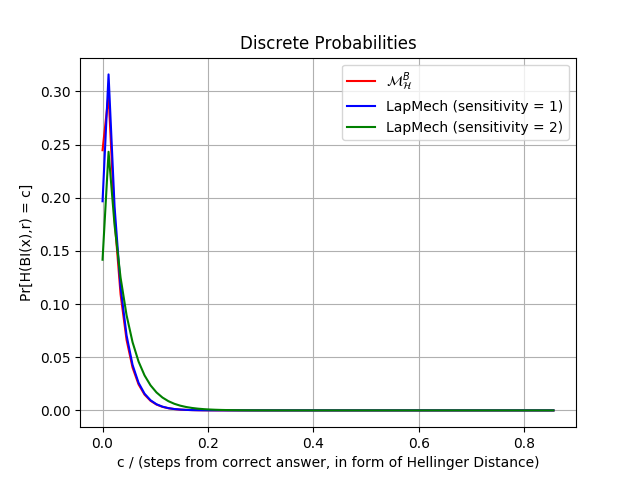
\includegraphics[width=0.328\textwidth]{poster_1.eps}
    \label{subfig_sampling_2d}
  }
  \subfigure[\footnotesize{3-dimensional, data size $\in [100,500]$} ]{
    \includegraphics[width=0.297\textwidth]{poster_2.eps}
  \label{subfig_sampling_3d}
  } 
  \subfigure[\footnotesize{4-dimensional, data size $\in [100,600]$}]{
    \includegraphics[width=0.29\textwidth]{poster_3.eps}
    \label{subfig_sampling_4d}
  }
  \caption{Increasing data size}
\label{fig_sampling}
\end{center}
\end{figure}

Fig. \ref{fig_concrete_prob} gives us the concrete probabilities of outputting candidates with certain Hellinegr distance from the correct posterior in 2, 3 and 4 dimensional respectively.
\begin{figure}[H]
\begin{center}
\centering
  \subfigure[2-dimensional]{
    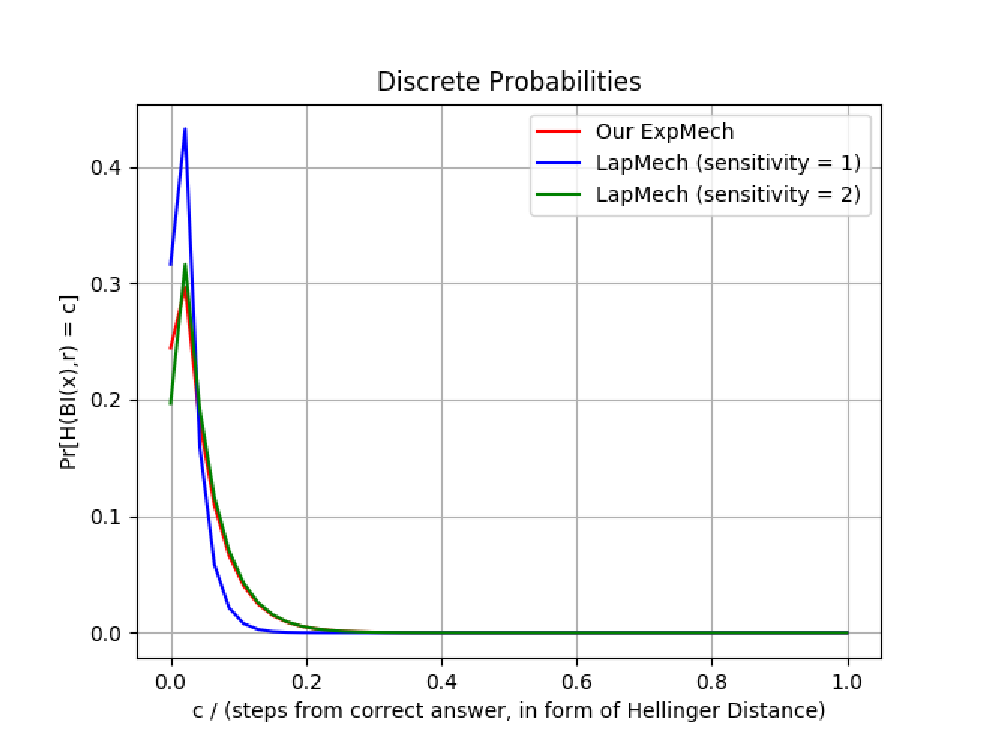
\includegraphics[width=0.31\textwidth]{poster_4.eps}
  \label{fig_concrete_prob_2d}
  }
  \subfigure[3-dimensional]{
    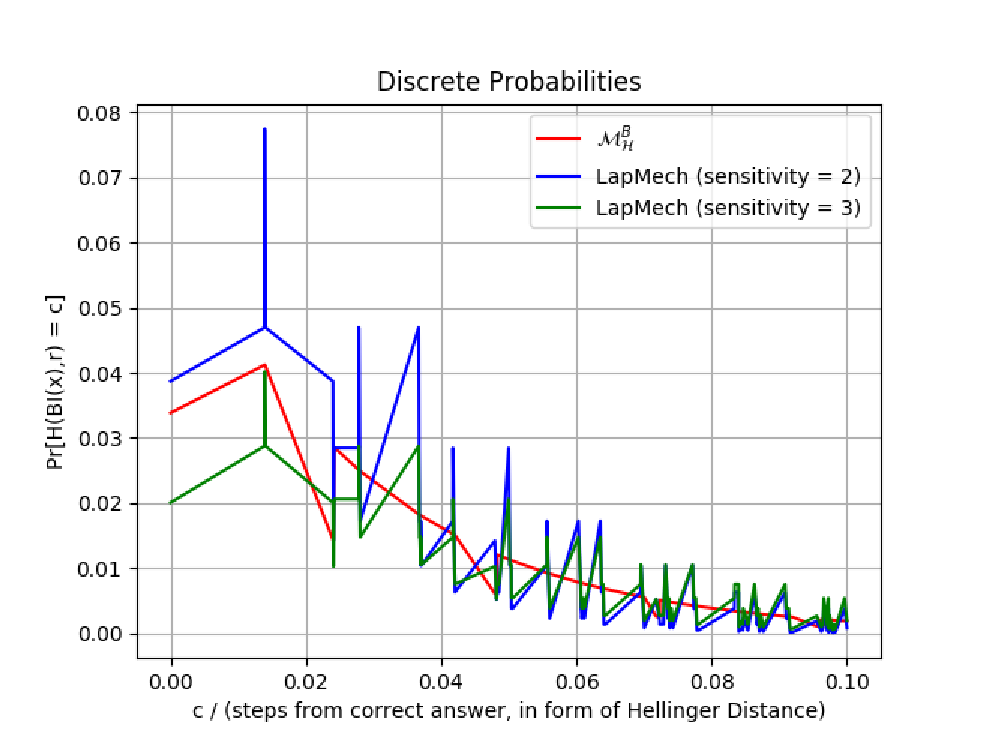
\includegraphics[width=0.31\textwidth]{poster_5.eps}
  \label{fig_concrete_prob_3d}
  } 
  \subfigure[4-dimensional]{
    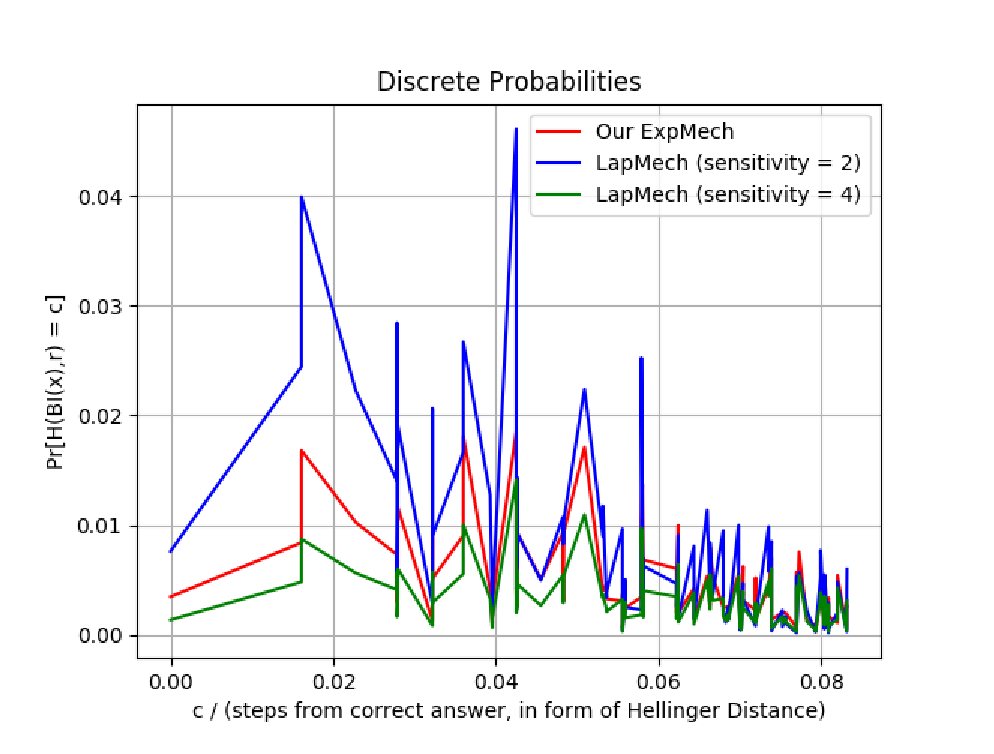
\includegraphics[width=0.31\textwidth]{poster_6.eps}
  \label{fig_concrete_prob_4d}
  } 
\caption{The concrete outputting probabilities under different dimensions with data set of size $600$}
\label{fig_concrete_prob}
\end{center}
\end{figure}
\scriptsize{Two groups of experiments both with unit prior $\betad(1,1), \betad(1,1,1)$ and $\betad(1,1,1,1)$, balanced datasets and parameters $\epsilon = 1.0$ and $\delta = 10^{-8}$.}
\end{block}


%----------------------------------------------------------------------------------------
% CONCLUSION
%----------------------------------------------------------------------------------------


\begin{block}{Conclusion}

\begin{itemize}
  \item The smoothed Hellinger distance based exponential mechanism outperforms the $\ell_1$-norm approach when data size growing under the case that Laplace noise doesn't have knowledge of the implicit histogram equivalence.
  % \begin{enumerate}
  %   \item  The accuracy that we are going to explore next, and in a more principled and formal way.
    
  %   \item  Experiments have shown that the actual privacy loss
  % in the experiments can be smaller than $\epsilon$. This means that we
  % could improve accuracy, by adding less noise but still achieve
  % $(\epsilon, \delta)$-dp.

  %   \item The choice of the Hellinger distance might seem quite ad-hoc. Hence, it is worth exploring other distances over distributions. An interesting class of probability metrics is the family of $f$-divergences \cite{CIT-004}.

  %   \item Other application of our scheme are going to be explored.
  % \end{enumerate}
\end{itemize}
%\vspace{8mm}
%\vspace{8mm}
%where we require $t$ and $u$ to have distinct sets of free variables.
\end{block}


%----------------------------------------------------------------------------------------
%	RESULTS
%----------------------------------------------------------------------------------------




%------------------------------------------------

% \begin{block}{Results: Figure}

% \begin{figure}
% 
\includegraphics[width=0.8\linewidth]{placeholder.jpg}
% \caption{Figure caption}
% \end{figure}

% \end{block}



%----------------------------------------------------------------------------------------
%	REFERENCES
%----------------------------------------------------------------------------------------

\begin{block}{References}
        
%\nocite{*} % Insert publications even if they are not cited in the poster
\small{\bibliographystyle{unsrt}
\bibliography{bayesian}}

\end{block}

%----------------------------------------------------------------------------------------
%	ACKNOWLEDGEMENTS
%----------------------------------------------------------------------------------------

% \begin{block}{Acknowledgments}

% \begin{itemize}
% \item Nam mollis tristique neque eu luctus. Suspendisse rutrum congue nisi sed convallis. Aenean id neque dolor. Pellentesque habitant morbi tristique senectus et netus et malesuada fames ac turpis egestas.
% \end{itemize}

% \end{block}

%----------------------------------------------------------------------------------------
%	CONTACT INFORMATION
%----------------------------------------------------------------------------------------

\setbeamercolor{block title}{fg=black,bg=orange!70} % Change the block title color

% \begin{block}{Contact Information}

% \begin{itemize}
% \item \textbf{Marco Gaboardi}
% \item Web: \href{http://staff.computing.dundee.ac.uk/marcogaboardi/}{http://staff.computing.dundee.ac.uk/marcogaboardi/}
% \item Email: \href{mailto:m.gaboardi@dundee.ac.uk}{m.gaboardi@dundee.ac.uk}
% %\item Phone: +1 617-384-9606
% \end{itemize}

% \end{block}

%----------------------------------------------------------------------------------------

\end{column} % End of the second column

\begin{column}{.01\textwidth}\end{column} % Empty spacer column

\end{columns} % End of all the columns in the poster

\end{frame} % End of the enclosing frame

\end{document}
